\documentclass[a4paper,12pt]{book}
\newcommand\tab[1][1cm]{\hspace*{#1}}
\usepackage{graphicx}
\usepackage{hyperref}
\usepackage{float}
\usepackage{adjustbox}
\usepackage{listings}
\graphicspath{ {./images/} }

\begin{document}
	
\author{Miłosz Wojciechowski}
\title{Stella-vslam installation manual for WSL}
\date{\today\\ v0.1}


\maketitle
\pagenumbering{arabic}
\tableofcontents

\mainmatter
\chapter{Environment preparation}
\section{Install WSL on your windows 10 system}
\begin{itemize}
	\item Open windows command prompt by typing cmd in start menu
	\item Write \textit{wsl \texttt{-{}-}install} (by default it will install the Ubuntu distribution of Linux, if you want to change that visit \href{https://learn.microsoft.com/en-us/windows/wsl/basic-commands#install}{this site})
	\item Just follow instructions displaying on the console, computer restart might be needed
	\item If you run into an issue during install process \href{https://learn.microsoft.com/en-us/windows/wsl/troubleshooting#installation-issues}{check this site}
\end{itemize}
\section{Prepare Ubuntu system}
\begin{itemize}
	\item type your username and password (remember it, since you will need this to work on this system)
	\item To turn copy/paste on just click on the Ubuntu icon in the left upper corner of the console
	\item \begin{minipage}[t]{\linewidth}
		\raggedright
		\adjustbox{valign=t}{%
			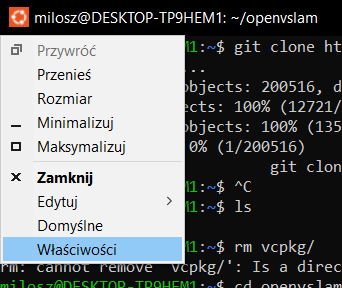
\includegraphics[width=.8\linewidth]{copy_paste1}%
		}
		
		\medskip
		Go to Properties.
	\end{minipage}
	\item \begin{minipage}[t]{\linewidth}
		\raggedright
		\adjustbox{valign=t}{%
			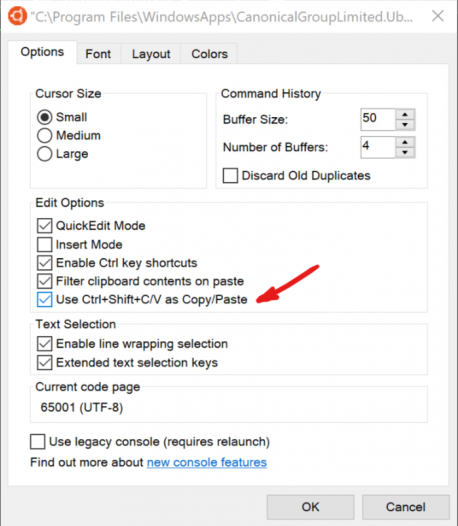
\includegraphics[width=.8\linewidth]{copy_paste2}%
		}
		
		\medskip
		Tick "Use Ctrl+Shift+C/V as Copy/Paste" option
	\end{minipage}
	\item Now search and install system updates by using commands:
	
	\vspace{3mm}
	sudo apt update -y
	
	\vspace{0.05mm}
	sudo apt upgrade -y \texttt{-{}-}no-install-recommends
	
	
	sudo apt install -y build-essential pkg-config git wget \\
	sudo apt install -y sqlite3 libsqlite3-dev
	\vspace{3mm}
	
	sudo apt-get install binutils-dev \\
	sudo apt-get install libdwarf-dev
	\item If you want to search WSL files with Windows File Explorer just type following path in your File Explorer:
	
	\vspace{3mm}
	\verb*|\\wsl$|
\end{itemize}
\section{Install CMake}
\begin{itemize}
	\item For safety uninstall CMake version if it was installed by default on Ubuntu:
	
	\vspace{3mm}
	sudo apt purge \texttt{-{}-}auto-remove cmake
	\vspace{3mm}
	
	\item Install CMake:
	
	\vspace{3mm}
	sudo apt-get install cmake
	\vspace{3mm}
\end{itemize}
\section{Install vcpkg}
\begin{itemize}
	\item First install zip and tar package:
	
	\vspace{3mm}
	sudo apt-get install curl zip unzip tar
	\vspace{3mm}
	
	\item Download vcpkg from GitHub:
	
	\vspace{3mm}
	wget -O vcpkg.tar.gz https://github.com/microsoft/vcpkg/archive/master.tar.gz
	\vspace{3mm}
	
	\item Create a new directory for vcpkg and unpack downloaded file there:
	
	\vspace{3mm}
	sudo mkdir /opt/vcpkg
	
	\vspace{0.05mm}
	sudo tar xf vcpkg.tar.gz \texttt{-{}-}strip-components=1 -C /opt/vcpkg
	\vspace{3mm}
	
	\item Now build vcpkg:
	
	\vspace{3mm}
	sudo /opt/vcpkg/bootstrap-vcpkg.sh
	\vspace{3mm}
	
	\item Make a symbolic link to the vcpkg command in “/usr/local/bin”:
	
	\vspace{3mm}
	sudo ln -s /opt/vcpkg/vcpkg /usr/local/bin/vcpkg
	\vspace{3mm}
	
	\item If you want to check the version of installed vcpkg use the following command:
	
	\vspace{3mm}
	vcpkg version
	\vspace{3mm}
	
	\item Lastly remove file downloaded from GitHub:
	
	\vspace{3mm}
	rm -rf vcpkg.tar.gz
	\vspace{3mm}
\end{itemize}

\chapter{Install libraries required by stella-vslam}
\section{Eigen}
\begin{itemize}
	\item To install Eigen use the following command:
	
	\vspace{3mm}
	sudo vcpkg install eigen3:x64-linux
	\vspace{3mm}
\end{itemize}
\section{g2o}
\begin{itemize}
	\item First install Fortran, to do this use the command:
	
	\vspace{3mm}
	sudo apt-get install gfortran
	\vspace{3mm}
	
	\item Now install g2o, x64-linux is added to be sure we are downloading 64-bit version of the library. g2o has many dependencies so installation may take a while:
	
	\vspace{3mm}
	sudo vcpkg install g2o:x64-linux
	\vspace{3mm}
\end{itemize}
\section{Yaml-cpp}
\begin{itemize}
	\item To install yaml-cpp use:
	
	\vspace{3mm}
	sudo vcpkg install yaml-cpp:x64-linux
	\vspace{3mm}
\end{itemize}
\section{OpenCV}
\begin{itemize}
	\item First install bison utility:
	
	\vspace{3mm}
	sudo apt-get update
	
	\vspace{0.05mm}
	sudo apt-get install bison
	\vspace{3mm}
	
	\item Now install libgtk2.0-dev:
	
	\vspace{3mm}
	sudo apt-get install libgtk2.0-dev
	\vspace{3mm}
	\item Install OpenCV3:
	
	\vspace{3mm}
	sudo vcpkg install opencv3:x64-linux
	\vspace{3mm}
\end{itemize}
\section{Pangolin}
\begin{itemize}
	\item Install nasm:
	
	\vspace{3mm}
	sudo apt-get install nasm
	\vspace{3mm}
	\item Install Glew:
	
	\vspace{3mm}
	sudo apt-get install libglew-dev
	\vspace{3mm}
	\item Install Pangolin:
	
	\vspace{3mm}
	sudo vcpkg install pangolin:x64-linux
	\vspace{3mm}
\end{itemize}
\section{FBoW}
\begin{itemize}
	\item Use the following commands to download and build the custom version of the library:
	
	\vspace{3mm}
	cd /tmp
	
	\vspace{0.05mm}
	git clone https://github.com/stella-cv/FBoW.git
	
	\vspace{0.05mm}
	cd FBoW
	
	\vspace{0.05mm}
	mkdir build \verb*|&&| cd build
	
	\vspace{0.05mm}
	cmake \textbackslash \\
	     \tab \verb*|-DCMAKE_BUILD_TYPE=Release| \textbackslash \\
	     \tab \verb*|-DCMAKE_INSTALL_PREFIX|=/usr/local \textbackslash \\ 
	     \tab -S ../  \verb*|-DBUILD_TESTS=ON| \verb*|-DBUILD_UTILS=ON| \textbackslash \\ 
	     \tab \verb*|-DCMAKE_TOOLCHAIN_FILE|=/opt/vcpkg/scripts/buildsystems/vcpkg.cmake
	
	\vspace{0.05mm}
	make -j4 \verb*|&&| sudo make install
\end{itemize}

\chapter{Stella-vslam installation}
\section{Build basic library}
\begin{itemize}
	\item mkdir -p \texttildelow/lib
	\item cd \texttildelow/lib
	\item git clone \texttt{-{}-}recursive https://github.com/stella-cv/\verb|stella_vslam|.git
	\item mkdir build \verb|&&| cd build
	\item cmake \verb|-DCMAKE_BUILD_TYPE|=RelWithDebInfo -S ../\verb|stella_vslam| \textbackslash \\ \verb|-DCMAKE_TOOLCHAIN_FILE|=/opt/vcpkg/scripts/buildsystems/vcpkg.cmake
	\item \textbf{SKIP TO MAKE -J4 IF CMAKE COMMAND WAS SUCCESSFUL}\\
	If previous command gives you error that some library installed via vcpkg wasn't detected perform the following step:\\
	Open CMakeLists.txt in ~/lib/\verb|stella_vslam| directory and paste the following line before \verb|find_package|()
	
	\vspace{1mm}
	include(/opt/vcpkg/scripts/buildsystems/vcpkg.cmake)
	\item \begin{minipage}[t]{\linewidth}
		\raggedright
		\adjustbox{valign=t}{%
			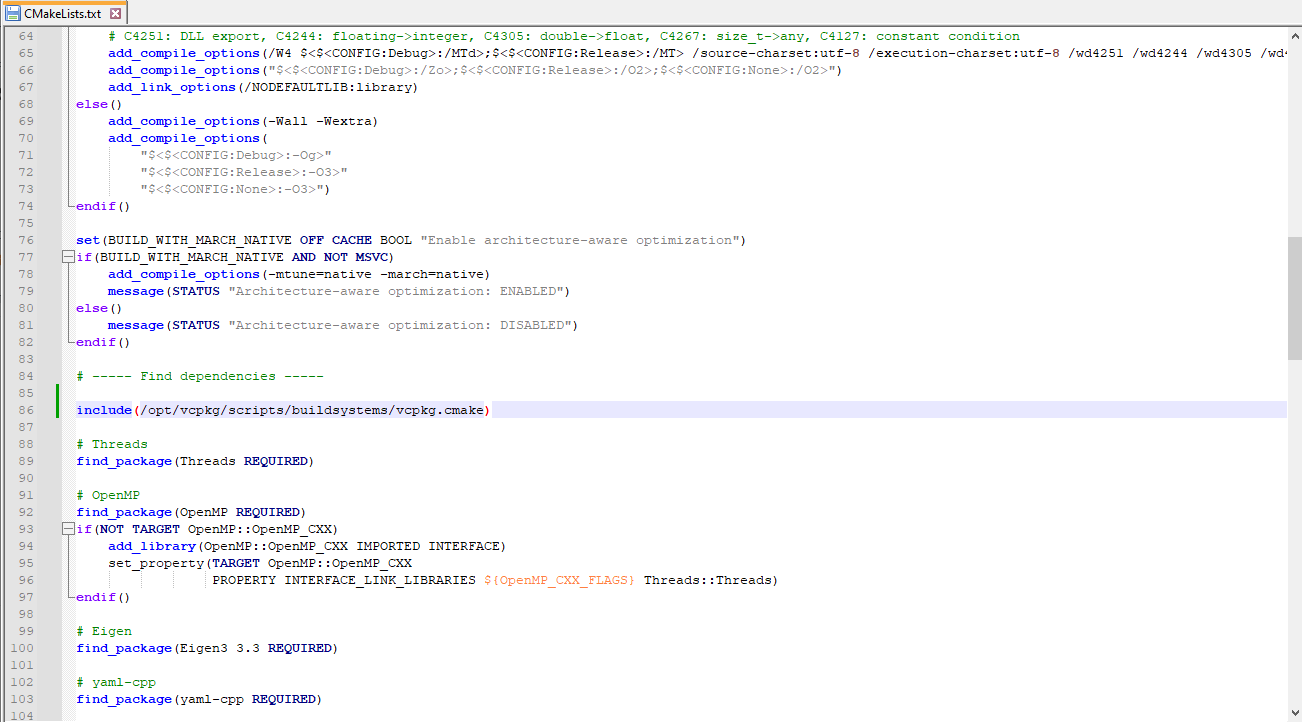
\includegraphics[width=.8\linewidth]{CMakeLists}%
		}
		
		\medskip
		It should look like this. 
	\end{minipage}
	
	Then run command: \\
	cmake \verb|-DCMAKE_BUILD_TYPE|=RelWithDebInfo -S ../\verb|stella_vslam|
	\item make -j4
	\item sudo make install
\end{itemize}
\section{Build with support for PangolinViewer}
\begin{itemize}
	\item cd \texttildelow/lib
	\item git clone -b 0.0.1 \texttt{-{}-}recursive https://github.com/stella-cv/\verb|pangolin_viewer|.git
	\item mkdir -p \verb|pangolin_viewer|/build
	\item cd \verb|pangolin_viewer|/build
	\item cmake \verb|-DCMAKE_BUILD_TYPE|=RelWithDebInfo -S ../ \textbackslash \\ \verb|-DCMAKE_TOOLCHAIN_FILE|=/opt/vcpkg/scripts/buildsystems/vcpkg.cmake
	\item \textbf{SKIP TO MAKE -J IF CMAKE COMMAND WAS SUCCESSFUL}\\ 
	If previous command gives you error that some library installed via vcpkg wasn't detected perform the following step:\\
	Open CMakeLists.txt in ~lib/\verb|pangolin_viewer| directory and paste the following line before \verb|find_package|()
	
	\vspace{1mm}
	include(/opt/vcpkg/scripts/buildsystems/vcpkg.cmake)\\
	
	Then run command:\\
	cmake \verb|-DCMAKE_BUILD_TYPE|=RelWithDebInfo -S ../
	
	\item make -j
	\item sudo make install
\end{itemize}
\section{Build examples}
\begin{itemize}
	\item Install Backward-cpp library:
	
	\vspace{3mm}
	sudo apt-get install libbackward-cpp-dev
	
	\item cd \texttildelow/lib
	\item git clone -b 0.0.1 \texttt{-{}-}recursive https://github.com/stella-cv/\verb|stella_vslam_examples|.git
	\item mkdir -p \verb|stella_vslam_examples|/build
	\item cd \verb|stella_vslam_examples|/build
	\item cmake \textbackslash \\
	\verb|-DCMAKE_BUILD_TYPE|=RelWithDebInfo \textbackslash \\
	\verb|-DUSE_STACK_TRACE_LOGGER|=ON \textbackslash \\
	-S ../ \verb|-DCMAKE_TOOLCHAIN_FILE|=/opt/vcpkg/scripts/buildsystems/vcpkg.cmake
	\item \textbf{SKIP TO MAKE -J IF CMAKE COMMAND WAS SUCCESSFUL}\\ 
	If previous command gives you error that some library installed via vcpkg wasn't detected perform the following step:\\
	Open CMakeLists.txt in ~lib/\verb|stella_vslam_examples| directory and paste the following line before \verb|find_package|()
	
	\vspace{1mm}
	include(/opt/vcpkg/scripts/buildsystems/vcpkg.cmake)\\
	
	Then run command: \\
	cmake \textbackslash \\
	\verb|-DCMAKE_BUILD_TYPE|=RelWithDebInfo \textbackslash \\
	\verb|-DUSE_STACK_TRACE_LOGGER|=ON \textbackslash \\
	-S ../
	\item make -j
	\item After building check if everything was successfully built:
	
	\vspace{3mm}
	./\verb|run_kitti_slam| -h
\end{itemize}
\end{document}